
\section{Regularization}

\begin{frame}{Regularization: Motivation}
    \only<1-4>{
        \begin{tikzpicture}
            \node[] at (-5.25, -3) {};
            \node[] at (5.25, 3) {};

            \only<1-2>{
                \node[anchor=west] at (-3.8, 2.5) {
                    $y \sim \beta_0 + \beta_1 * x_1 + \beta_2 * x_2$
                };
            }
            \only<3>{
                \node[anchor=west] at (-3.8, 2.5) {
                    $y \sim \beta_0 + \beta_1 * x_1 + \beta_2 * x_2 + \beta_3 * x_3 + \beta_4 * x_4$
                };
            }

            \only<2-3>{
                \node[draw=black, fill=white] at (0, -0.5){
                    \includegraphics[width=8cm]{data/overfitting.png}
                };
            }

            \only<4>{
                \PythonInputNode{1}{(-4, 2)}{code}{0.9\textwidth}{7}{
                    import pandas as pd^^J
                    ^^J
                    ^^J
                    df = pd.read_csv('/Users/esten/Downloads/Auto.csv')^^J
                    train = df.iloc[:int(len(df) * 0.8)]^^J
                    validation = df.iloc[int(len(df) * 0.8):]^^J
                    ^^J
                    print(f'Using {len(train)} samples for training')^^J
                    print(f'Using {len(validation)} samples for validation')^^J
                }
                \PythonOutputNode{1}{($ (code.south west) + (0.11, -0.2) $)}{output}{0.791\textwidth}{7}{
                    Using 317 samples for training^^J
                    Using 80 samples for validation^^J
                }
            }
        \end{tikzpicture}
    }
    \only<5-6>{
        \begin{enumerate}
            \item Variable selection
            \begin{enumerate}
                \item[a.] Best subset selection
                \item[b.] Forward stepwise selection
                \item[c.] Backward stepwise selection
            \end{enumerate}
            \item Shrinkage
            \begin{enumerate}
                \alert<6>{\item[a.] LASSO}
                \alert<6>{\item[b.] Ridge Regression}
            \end{enumerate}
            \item Dimensionality reduction: Lecture 6 and self-study
        \end{enumerate}
    }
\end{frame}

\section{Variable selection}

\newcommand{\autoplot}[1]{
    \nextgroupplot[
        title=\scriptsize{#1},
        every axis title/.style={at={(0.5,1.15)}},
        xmajorticks=false,
        xmajorgrids=true,
        ymajorticks=false,
        ymajorgrids=true
    ]
        \addplot[
            only marks,
            mark=*,
            color=blue,
            opacity=0.25
        ] table[
            col sep=comma,
            y=mpg,
            x=#1
        ] {data/Auto.csv};
}

\newsavebox{\predictors}
\sbox{\predictors}{
    \begin{tikzpicture}
        \begin{groupplot}[
            group style={
                group size=3 by 2,
                horizontal sep=0.5cm
            },
            ticklabel style = {font=\tiny},
            height=3.9cm,
            width=3.9cm
        ]
            \autoplot{cylinders}
            \autoplot{displacement}
            \autoplot{horsepower}
            \autoplot{weight}
            \autoplot{acceleration}
            \autoplot{year}
        \end{groupplot}
    \end{tikzpicture}
}

\begin{frame}{Variable selection}
    \begin{tikzpicture}
        \node[] at (-5.25, -3) {};
        \node[] at (5.25, 3) {};

        \only<1>{
            \node[align=center, text width=10cm, align=flush center] at (0, 0) {
                The number of predictors we are using in our model directly impacts model complexity.
            };
        }
        \only<2-4>{
            \node[align=flush left, anchor=west, text width=10cm] at (-5.2, 2.5) {
                \textbf{Problem}\\
                We have a set of predictors $P=\{x_0, x_1, ...\}$ and a target variable $y$, and we want to find the subset $p \subseteq P$ that yields the best (linear) model for predicting $y$.
            };
        }
        \only<3-4>{
            \node[align=flush left, anchor=west, text width=10cm] at (-5.2, 0) {
                \textbf{Motivation}\\
                To reduce model complexity (and therefore risk of overfitting), \alert<4>{avoid problems due to collinearity}, and simplify subsequent interpretations.
            };
        }
        \only<5>{
            \node[] at (0, 0) {
                \usebox{\predictors}
            };
        }
    \end{tikzpicture}
\end{frame}

\begin{frame}[t]{Variable selection: Best subset selection}
    \only<1,4>{
        \textbf{Problem}\\
        We have a set of predictors $P=\{x_0, x_1, ...\}$ and a target variable $y$, and we want to find the subset $p \subseteq P$ that yields the best (linear) model for predicting $y$.\\
        \vspace{0.25cm}
        \textbf{Solution}\\
        Train models on all subsets $p$ and select the best one.
    }
    \only<2-3>{
        \begin{tikzpicture}
            \node[] at (-5.25, -3) {};
            \node[] at (5.25, 3) {};

            \PythonInputNode{1}{(-5, 2.5)}{code}{0.95\textwidth}{6}{
import numpy as np^^J
^^J
from itertools import chain, combinations^^J
from sklearn.linear_model import LinearRegression^^J
from sklearn.metrics import mean_squared_error^^J
^^J
subsets = list(chain.from_iterable(combinations(predictors, r) \^^J
{ }{ }{ }{ }{ }{ }{ }{ }{ }{ }{ }{ }{ }{ }{ }for r in range(len(predictors)+1)))^^J
^^J
best = \{'mse': float('inf'), 'subset': None\}^^J
^^J
for subset in subsets:^^J
{ }{ }{ }{ }if len(subset) == 0:^^J
{ }{ }{ }{ }{ }{ }{ }{ }continue^^J
^^J
{ }{ }{ }{ }model = LinearRegression()^^J
{ }{ }{ }{ }model.fit(train[list(subset)], train[target])^^J
{ }{ }{ }{ }predictions = model.predict(validation[list(subset)])^^J
{ }{ }{ }{ }mse = mean_squared_error(validation[target], predictions)^^J
^^J
{ }{ }{ }{ }best = best if mse > best['mse'] else  \{'mse': mse, 'subset': subset\}^^J
^^J
print(f'MSE: \{best["mse"]:.2f\}, predictors: \{best["subset"]\}')^^J
            }
            \PythonOutputNode{1}{($ (code.south west) + (0.11, -0.2) $)}{output}{0.881\textwidth}{6}{
MSE: 29.68, predictors: ('cylinders', 'displacement', 'horsepower', 'weight', 'year')^^J
            }

        \only<3>{
            \node[draw=red, thick, minimum height=0.3cm, minimum width=1.9cm] at (-1.9, -2.55) {};
        }
        \end{tikzpicture}
    }
    \only<4>{
        %\vspace{0.25cm}

        \textcolor{green}{+} \textbf{Positives}\\
        \textbullet{ }Guaranteed to find the optimal solution.\\
        \textbullet{ }Simple implementation\\
        %\vspace{0.25cm}

        \textcolor{red}{-} \textbf{Drawbacks}\\
        \textbullet{ }Need to train many ($2^{|P|}$) models.
    }
    \only<5>{
        \centering
        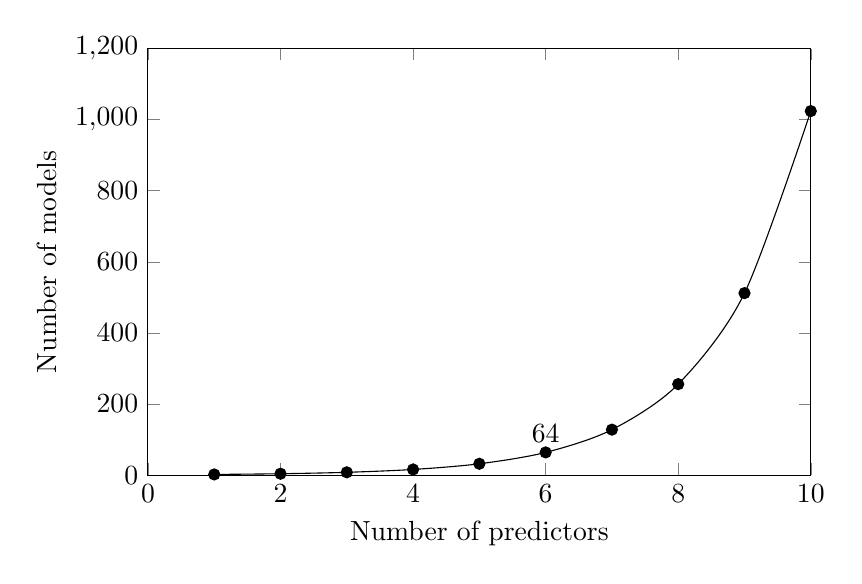
\begin{tikzpicture}
            \begin{axis}[
                smooth,
                xmin=0,
                xmax=10,
                ymin=0,
                ymax=1200,
                xlabel={Number of predictors},
                ylabel={Number of models},
                height=7cm,
                width=10cm
            ]
                \addplot[mark=*] coordinates {
                    (1, 2^1)
                    (2, 2^2)
                    (3, 2^3)
                    (4, 2^4)
                    (5, 2^5)
                    (6, 2^6)
                    (7, 2^7)
                    (8, 2^8)
                    (9, 2^9)
                    (10, 2^10)
                };
                \node[anchor=south] at (axis cs: 6, 2^6) {64};
            \end{axis}
        \end{tikzpicture}
    }
\end{frame}

 \begin{frame}[t]{Variable selection: Forward stepwise selection}
    \only<1-2,13>{
        \textbf{Problem}\\
        We have a set of predictors $P=\{x_0, x_1, ...\}$ and a target variable $y$, and we want to find the subset $p \subseteq P$ that yields the best (linear) model for predicting $y$.\\
        \vspace{0.25cm}
        \textbf{Solution}\\
        Start with no predictors. Iteratively add the predictor that yields the \alert<2>{best model} until all are included.\\

        \only<13>{
            \vspace{0.25cm}
            \textcolor{green}{+}{ }\textbf{Positives}\\
            \textbullet{ }Need to train fewer models.\\
            \vspace{0.25cm}
            \textcolor{red}{-}{ }\textbf{Drawbacks}\\
            \textbullet{ }Not guaranteed to find the optimal solution.\\
        }
    }

    \only<3-10>{
        \def\nodefont{\fontsize{4}{4}\linespread{0.85}\selectfont}
        \def\hsep{1.6}
        \def\vsep{0.75}
        \begin{tikzpicture}
            \node[draw=black, align=center, font=\nodefont] (n00) at (0, 0 * \vsep) {
                $y \sim \mathbbm{1}$\\
                $mse=146.47$
            };

            \node[] at (6.5 * \hsep, 3.3 * \vsep) {};
            \node[] at (-0.32 * \hsep, -3.3 * \vsep) {};

            \only<4>{
                \node[draw=black, align=center, font=\nodefont, color=black] (n11) at (\hsep, 2.5 * \vsep) {
                    $y \sim cylinders$\\
                    $67.96$
                };
                \node[draw=black, align=center, font=\nodefont, color=black] (n12) at (\hsep, 1.5 * \vsep) {
                    $y \sim year$\\
                    $61.56$
                };
                \node[draw=black, align=center, font=\nodefont, color=black] (n13) at (\hsep, 0.5 * \vsep) {
                    $y \sim acceleration$\\
                    $119.72$
                };
                \node[draw=black, align=center, font=\nodefont] (n14) at (\hsep, -0.5 * \vsep) {
                    $y \sim weight$\\
                    $61.18$
                };
                \node[draw=black, align=center, font=\nodefont, color=black] (n15) at (\hsep, -1.5 * \vsep) {
                    $y \sim horsepower$\\
                    $65.75$
                };
                \node[draw=black, align=center, font=\nodefont, color=black] (n16) at (\hsep, -2.5 * \vsep) {
                    $y \sim displacement$\\
                    $63.84$
                };


                \draw[black] (n00.east) -- (n11.west);
                \draw[black] (n00.east) -- (n12.west);
                \draw[black] (n00.east) -- (n13.west);
                \draw[black] (n00.east) -- (n14.west);
                \draw[black] (n00.east) -- (n15.west);
                \draw[black] (n00.east) -- (n16.west);
            }
            \only<5-10>{
                \node[draw=gray!25, align=center, font=\nodefont, color=gray!25] (n11) at (\hsep, 2.5 * \vsep) {
                    $y \sim cylinders$\\
                    $67.96$
                };
                \node[draw=gray!25, align=center, font=\nodefont, color=gray!25] (n12) at (\hsep, 1.5 * \vsep) {
                    $y \sim year$\\
                    $61.56$
                };
                \node[draw=gray!25, align=center, font=\nodefont, color=gray!25] (n13) at (\hsep, 0.5 * \vsep) {
                    $y \sim acceleration$\\
                    $119.72$
                };
                \node[draw=black, align=center, font=\nodefont] (n14) at (\hsep, -0.5 * \vsep) {
                    $y \sim weight$\\
                    $61.18$
                };
                \node[draw=gray!25, align=center, font=\nodefont, color=gray!25] (n15) at (\hsep, -1.5 * \vsep) {
                    $y \sim horsepower$\\
                    $65.75$
                };
                \node[draw=gray!25, align=center, font=\nodefont, color=gray!25] (n16) at (\hsep, -2.5 * \vsep) {
                    $y \sim displacement$\\
                    $63.84$
                };


                \draw[gray!25] (n00.east) -- (n11.west);
                \draw[gray!25] (n00.east) -- (n12.west);
                \draw[gray!25] (n00.east) -- (n13.west);
                \draw[black] (n00.east) -- (n14.west);
                \draw[gray!25] (n00.east) -- (n15.west);
                \draw[gray!25] (n00.east) -- (n16.west);
            }
            \only<6>{
                \node[draw=black, align=center, font=\nodefont, color=black] (n21) at (2 * \hsep, 2.5 * \vsep) {
                    $\begin{aligned}
                        y\sim&weight +\\[-0.8em]
                        &cylinders
                    \end{aligned}$\\
                    $60.02$
                };
                \node[draw=black, align=center, font=\nodefont] (n22) at (2 * \hsep, 1.25 * \vsep) {
                    $\begin{aligned}
                        y\sim&weight +\\[-0.8em]
                        &year
                    \end{aligned}$\\
                    $29.84$
                };
                \node[draw=black, align=center, font=\nodefont, color=black] (n23) at (2 * \hsep, 0 * \vsep) {
                    $\begin{aligned}
                        y\sim&weight +\\[-0.8em]
                        &acceleration
                    \end{aligned}$\\
                    $60.01$
                };
                \node[draw=black, align=center, font=\nodefont, color=black] (n24) at (2 * \hsep, -1.25 * \vsep) {
                    $\begin{aligned}
                        y\sim&weight +\\[-0.8em]
                        &horsepower
                    \end{aligned}$\\
                    $58.59$
                };
                \node[draw=black, align=center, font=\nodefont, color=black] (n25) at (2 * \hsep, -2.5 * \vsep) {
                    $\begin{aligned}
                        y\sim&weight +\\[-0.8em]
                        &displacement
                    \end{aligned}$\\
                    $59.91$
                };

                \draw[black] (n14.east) -- (n21.west);
                \draw[black] (n14.east) -- (n22.west);
                \draw[black] (n14.east) -- (n23.west);
                \draw[black] (n14.east) -- (n24.west);
                \draw[black] (n14.east) -- (n25.west);
            }
            \only<7-10>{
                \node[draw=gray!25, align=center, font=\nodefont, color=gray!25] (n21) at (2 * \hsep, 2.5 * \vsep) {
                    $\begin{aligned}
                        y\sim&weight +\\[-0.8em]
                        &cylinders
                    \end{aligned}$\\
                    $60.02$
                };
                \node[draw=black, align=center, font=\nodefont] (n22) at (2 * \hsep, 1.25 * \vsep) {
                    $\begin{aligned}
                        y\sim&weight +\\[-0.8em]
                        &year
                    \end{aligned}$\\
                    $29.84$
                };
                \node[draw=gray!25, align=center, font=\nodefont, color=gray!25] (n23) at (2 * \hsep, 0 * \vsep) {
                    $\begin{aligned}
                        y\sim&weight +\\[-0.8em]
                        &acceleration
                    \end{aligned}$\\
                    $60.01$
                };
                \node[draw=gray!25, align=center, font=\nodefont, color=gray!25] (n24) at (2 * \hsep, -1.25 * \vsep) {
                    $\begin{aligned}
                        y\sim&weight +\\[-0.8em]
                        &horsepower
                    \end{aligned}$\\
                    $58.59$
                };
                \node[draw=gray!25, align=center, font=\nodefont, color=gray!25] (n25) at (2 * \hsep, -2.5 * \vsep) {
                    $\begin{aligned}
                        y\sim&weight +\\[-0.8em]
                        &displacement
                    \end{aligned}$\\
                    $59.91$
                };

                \draw[gray!25] (n14.east) -- (n21.west);
                \draw[black] (n14.east) -- (n22.west);
                \draw[gray!25] (n14.east) -- (n23.west);
                \draw[gray!25] (n14.east) -- (n24.west);
                \draw[gray!25] (n14.east) -- (n25.west);
            }
            \only<7>{
                \node[draw=black, align=center, font=\nodefont, color=black] (n31) at (3 * \hsep, 2.25 * \vsep) {
                    $\begin{aligned}
                        y\sim&weight +\\[-0.8em]
                        &year +\\[-0.8em]
                        &cylinders
                    \end{aligned}$\\
                    $29.91$
                };
                \node[draw=black, align=center, font=\nodefont, color=black] (n32) at (3 * \hsep, 0.75 * \vsep) {
                    $\begin{aligned}
                        y\sim&weight +\\[-0.8em]
                        &year +\\[-0.8em]
                        &acceleration
                    \end{aligned}$\\
                    $29.99$
                };
                \node[draw=black, align=center, font=\nodefont] (n33) at (3 * \hsep, -0.75 * \vsep) {
                    $\begin{aligned}
                        y\sim&weight +\\[-0.8em]
                        &year +\\[-0.8em]
                        &horsepower
                    \end{aligned}$\\
                    $29.85$
                };
                \node[draw=black, align=center, font=\nodefont, color=black] (n34) at (3 * \hsep, -2.25 * \vsep) {
                    $\begin{aligned}
                        y\sim&weight +\\[-0.8em]
                        &year +\\[-0.8em]
                        &displacement
                    \end{aligned}$\\
                    $29.96$
                };

                \draw[black] (n22.east) -- (n31.west);
                \draw[black] (n22.east) -- (n32.west);
                \draw[black] (n22.east) -- (n33.west);
                \draw[black] (n22.east) -- (n34.west);
            }
            \only<8-10>{
                \node[draw=gray!25, align=center, font=\nodefont, color=gray!25] (n31) at (3 * \hsep, 2.25 * \vsep) {
                    $\begin{aligned}
                        y\sim&weight +\\[-0.8em]
                        &year +\\[-0.8em]
                        &cylinders
                    \end{aligned}$\\
                    $29.91$
                };
                \node[draw=gray!25, align=center, font=\nodefont, color=gray!25] (n32) at (3 * \hsep, 0.75 * \vsep) {
                    $\begin{aligned}
                        y\sim&weight +\\[-0.8em]
                        &year +\\[-0.8em]
                        &acceleration
                    \end{aligned}$\\
                    $29.99$
                };
                \node[draw=black, align=center, font=\nodefont] (n33) at (3 * \hsep, -0.75 * \vsep) {
                    $\begin{aligned}
                        y\sim&weight +\\[-0.8em]
                        &year +\\[-0.8em]
                        &horsepower
                    \end{aligned}$\\
                    $29.85$
                };
                \node[draw=gray!25, align=center, font=\nodefont, color=gray!25] (n34) at (3 * \hsep, -2.25 * \vsep) {
                    $\begin{aligned}
                        y\sim&weight +\\[-0.8em]
                        &year +\\[-0.8em]
                        &displacement
                    \end{aligned}$\\
                    $29.96$
                };

                \draw[gray!25] (n22.east) -- (n31.west);
                \draw[gray!25] (n22.east) -- (n32.west);
                \draw[black] (n22.east) -- (n33.west);
                \draw[gray!25] (n22.east) -- (n34.west);
            }
            \only<8>{
                \node[draw=black, align=center, font=\nodefont, color=black] (n41) at (4 * \hsep, 1.75 * \vsep) {
                    $\begin{aligned}
                        y\sim&weight +\\[-0.8em]
                        &year +\\[-0.8em]
                        &horsepower +\\[-0.8em]
                        &cylinders
                    \end{aligned}$\\
                    $29.87$
                };
                \node[draw=black, align=center, font=\nodefont, color=black] (n42) at (4 * \hsep, 0 * \vsep) {
                    $\begin{aligned}
                        y\sim&weight +\\[-0.8em]
                        &year +\\[-0.8em]
                        &horsepower +\\[-0.8em]
                        &acceleration
                    \end{aligned}$\\
                    $30.29$
                };
                \node[draw=black, align=center, font=\nodefont, color=black] (n43) at (4 * \hsep, -1.75 * \vsep) {
                    $\begin{aligned}
                        y\sim&weight +\\[-0.8em]
                        &year +\\[-0.8em]
                        &horsepower +\\[-0.8em]
                        &displacement
                    \end{aligned}$\\
                    $29.95$
                };

                \draw[black] (n33.east) -- (n41.west);
                \draw[black] (n33.east) -- (n42.west);
                \draw[black] (n33.east) -- (n43.west);
            }
            \only<9-10>{
                \node[draw=black, align=center, font=\nodefont, color=black] (n41) at (4 * \hsep, 1.75 * \vsep) {
                    $\begin{aligned}
                        y\sim&weight +\\[-0.8em]
                        &year +\\[-0.8em]
                        &horsepower +\\[-0.8em]
                        &cylinders
                    \end{aligned}$\\
                    $29.87$
                };
                \node[draw=gray!25, align=center, font=\nodefont, color=gray!25] (n42) at (4 * \hsep, 0 * \vsep) {
                    $\begin{aligned}
                        y\sim&weight +\\[-0.8em]
                        &year +\\[-0.8em]
                        &horsepower +\\[-0.8em]
                        &acceleration
                    \end{aligned}$\\
                    $30.29$
                };
                \node[draw=gray!25, align=center, font=\nodefont, color=gray!25] (n43) at (4 * \hsep, -1.75 * \vsep) {
                    $\begin{aligned}
                        y\sim&weight +\\[-0.8em]
                        &year +\\[-0.8em]
                        &horsepower +\\[-0.8em]
                        &displacement
                    \end{aligned}$\\
                    $29.95$
                };

                \draw[black] (n33.east) -- (n41.west);
                \draw[gray!25] (n33.east) -- (n42.west);
                \draw[gray!25] (n33.east) -- (n43.west);
            }
            \only<9>{
                \node[draw=black, align=center, font=\nodefont] (n51) at (5 * \hsep, 1 * \vsep) {
                    $\begin{aligned}
                        y\sim&weight +\\[-0.8em]
                        &year +\\[-0.8em]
                        &horsepower +\\[-0.8em]
                        &cylinders +\\[-0.8em]
                        &acceleration
                    \end{aligned}$\\
                    $29.68$
                };
                \node[draw=black, align=center, font=\nodefont, color=black] (n52) at (5 * \hsep, -1 * \vsep) {
                    $\begin{aligned}
                        y\sim&weight +\\[-0.8em]
                        &year +\\[-0.8em]
                        &horsepower +\\[-0.8em]
                        &cylinders +\\[-0.8em]
                        &displacement
                    \end{aligned}$\\
                    $30.47$
                };

                \draw[black] (n41.east) -- (n51.west);
                \draw[black] (n41.east) -- (n52.west);
            }
            \only<10>{
                \node[draw=black, align=center, font=\nodefont] (n51) at (5 * \hsep, 1 * \vsep) {
                    $\begin{aligned}
                        y\sim&weight +\\[-0.8em]
                        &year +\\[-0.8em]
                        &horsepower +\\[-0.8em]
                        &cylinders +\\[-0.8em]
                        &acceleration
                    \end{aligned}$\\
                    $29.68$
                };
                \node[draw=gray!25, align=center, font=\nodefont, color=gray!25] (n52) at (5 * \hsep, -1 * \vsep) {
                    $\begin{aligned}
                        y\sim&weight +\\[-0.8em]
                        &year +\\[-0.8em]
                        &horsepower +\\[-0.8em]
                        &cylinders +\\[-0.8em]
                        &displacement
                    \end{aligned}$\\
                    $30.47$
                };

                \draw[black] (n41.east) -- (n51.west);
                \draw[gray!25] (n41.east) -- (n52.west);

                \node[draw=black, align=center, font=\nodefont] (n61) at (6 * \hsep, 0 * \vsep) {
                    $\begin{aligned}
                        y\sim&weight +\\[-0.8em]
                        &year +\\[-0.8em]
                        &horsepower +\\[-0.8em]
                        &cylinders +\\[-0.8em]
                        &acceleration +\\[-0.8em]
                        &displacement
                    \end{aligned}$\\
                    $30.29$
                };

                \draw[black] (n51.east) -- (n61.west);
            }
        \end{tikzpicture}
    }
    \only<11>{
        \centering
        \vspace{0.7cm}
        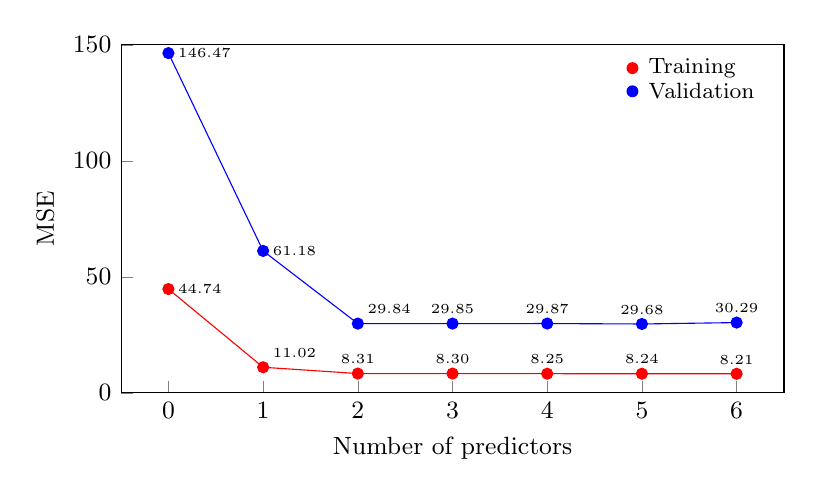
\begin{tikzpicture}
            \begin{axis}[
                xmin=-0.5,
                xmax=6.5,
                ymin=0,
                ymax=150,
                height=6cm,
                width=10cm,
                ytick pos=left,
                xtick pos=bottom,
                ylabel=\small{MSE},
                xlabel=\small{Number of predictors},
                ticklabel style={font=\small},
            ]
                \addplot[red,mark=*] coordinates {
                    (0, 44.74)
                    (1, 11.02)
                    (2, 8.31)
                    (3, 8.31)
                    (4, 8.25)
                    (5, 8.24)
                    (6, 8.21)
                };
                \addplot[blue,mark=*] coordinates {
                    (0, 146.47)
                    (1, 61.18)
                    (2, 29.84)
                    (3, 29.85)
                    (4, 29.87)
                    (5, 29.68)
                    (6, 30.29)
                };

                \node[
                    circle,
                    fill=red,
                    minimum size=4.3pt,
                    inner sep=0pt,
                    label=right:\footnotesize{Training}
                ] at (axis cs: 4.9, 140) {};
                \node[
                    circle,
                    fill=blue,
                    minimum size=4.3pt,
                    inner sep=0pt,
                    label=right:\footnotesize{Validation}
                ] at (axis cs: 4.9, 130) {};

                \node[anchor=west,font=\tiny] at (axis cs: 0, 44.74) {44.74};
                \node[anchor=south west,font=\tiny] at (axis cs: 1, 11.02) {11.02};
                \node[anchor=south,font=\tiny] at (axis cs: 2, 8.31) {8.31};
                \node[anchor=south,font=\tiny] at (axis cs: 3, 8.31) {8.30};
                \node[anchor=south,font=\tiny] at (axis cs: 4, 8.25) {8.25};
                \node[anchor=south,font=\tiny] at (axis cs: 5, 8.24) {8.24};
                \node[anchor=south,font=\tiny] at (axis cs: 6, 8.21) {8.21};

                \node[anchor=west,font=\tiny] at (axis cs: 0, 146.47) {146.47};
                \node[anchor=west,font=\tiny] at (axis cs: 1, 61.18) {61.18};
                \node[anchor=south west,font=\tiny] at (axis cs: 2, 29.84) {29.84};
                \node[anchor=south,font=\tiny] at (axis cs: 3, 29.85) {29.85};
                \node[anchor=south,font=\tiny] at (axis cs: 4, 29.87) {29.87};
                \node[anchor=south,font=\tiny] at (axis cs: 5, 29.68) {29.68};
                \node[anchor=south,font=\tiny] at (axis cs: 6, 30.29) {30.29};

            \end{axis}
        \end{tikzpicture}
    }
    \only<12>{
        \begin{tikzpicture}
            \node[] at (-5.25, -3) {};
            \node[] at (5.25, 3) {};

            \PythonInputNode{1}{(-5, 2.5)}{code}{0.95\textwidth}{4}{
def fit_and_evaluate(train: pd.DataFrame, validation: pd.DataFrame,^^J
{ }{ }{ }{ }{ }{ }{ }{ }{ }{ }{ }{ }{ }{ }{ }{ }{ }{ }{ }{ }{ }predictors: List[str], target: str):^^J
{ }{ }{ }{ }model = LinearRegression()^^J
{ }{ }{ }{ }model.fit(train[predictors], train[target])^^J
^^J
{ }{ }{ }{ }train_predictions = model.predict(train[predictors])^^J
{ }{ }{ }{ }validation_predictions = model.predict(validation[predictors])^^J
^^J
{ }{ }{ }{ }return np.mean((train_predictions - train[target]) ** 2), \^^J
{ }{ }{ }{ }{ }{ }{ }{ }{ }{ }{ }np.mean((validation_predictions - validation[target]) ** 2)^^J
^^J
^^J
predictors = ['cylinders', 'displacement', 'horsepower', 'weight', 'acceleration', 'year']^^J
target = 'mpg'^^J
^^J
train['intercept'] = 1^^J
validation['intercept'] = 1^^J
train_mse, validation_mse = fit_and_evaluate(train, validation, predictors=['intercept'], target=target)^^J
print(f'[]: \{validation_mse:.2f\} (\{train_mse:.2f\})')^^J
^^J
chosen_predictors = []^^J
^^J
while len(chosen_predictors) < len(predictors):^^J
{ }{ }{ }{ }best_predictor = \{'train_mse': None, 'validation_mse': float('inf'),^^J
{ }{ }{ }{ }{ }{ }{ }{ }{ }{ }{ }{ }{ }{ }{ }{ }{ }{ }{ }{ }{ }{ }'predictor': None\}^^J
      ^^J
{ }{ }{ }{ }for predictor in set(predictors) - set(chosen_predictors):^^J
{ }{ }{ }{ }{ }{ }{ }{ }train_mse, validation_mse = fit_and_evaluate(train, validation, predictors=chosen_predictors + [predictor], target=target)^^J
^^J
{ }{ }{ }{ }{ }{ }{ }{ }if validation_mse < best_predictor['validation_mse']:^^J
{ }{ }{ }{ }{ }{ }{ }{ }{ }{ }{ }{ }best_predictor = \{'train_mse': train_mse, 'validation_mse': validation_mse, 'predictor': predictor\}^^J
^^J
{ }{ }{ }{ }chosen_predictors.append(best_predictor['predictor'])^^J
^^J
{ }{ }{ }{ }print(f'\{chosen_predictors\}: \{best_predictor["validation_mse"]:.2f\} (\{best_predictor["train_mse"]:.2f\})')^^J
            }
        \end{tikzpicture}
    }
\end{frame}

\begin{frame}[t]{Variable selection: Backward stepwise selection}
    \only<1-2>{
        \textbf{Problem}\\
        We have a set of predictors $P=\{x_0, x_1, ...\}$ and a target variable $y$, and we want to find the subset $p \subseteq P$ that yields the best (linear) model for predicting $y$.\\
        \vspace{0.25cm}
        \textbf{Solution}\\
        Start with \alert<2>{all} predictors. Iteratively \alert<2>{remove} the predictor that yields the best model until all you have none left.\\
        \vspace{0.25cm}
        \textcolor{green}{+} \textbf{Positives}\\
        \textbullet{ }Need to train fewer models.\\
        \vspace{0.25cm}
        \textcolor{red}{-} \textbf{Drawbacks}\\
        \textbullet{ }Not guaranteed to find the optimal solution.\\
    }
    \only<3>{
        \vspace{3cm}
        \centering
        Does forward and backward stepwise selection yield the same set of predictors?
    }
\end{frame}

\section{Shrinkage}

\def\codewidth{5.2cm}

\begin{frame}{Shrinkage: Outline}
    \definecolor{mse}{HTML}{cc79a7}
    \definecolor{variance}{HTML}{10a47b}
    \begin{tikzpicture}
        \node[] at (-5.25, 3.5) {};
        \node[] at (5.25, -3.5) {};

        \only<1-5, 7-9>{
            \node[] at (0, 3) {
                $y \sim \beta_0 + \alert<2-9>{\beta_1}x_1 + \alert<2-9>{\beta_2}x_2 + \alert<2-9>{\beta_3}x_3 + \alert<2-9>{\beta_4}x_4 + \alert<2-9>{\beta_5}x_5 + \beta_6x_6$
            };
        }
        \only<3-5, 7-9>{
            \node[] at (0, 2.25) {
                \textcolor{orange}{$\beta_n \rightarrow 0$}
            };
        }
        \only<4-5, 7-8>{
            \node[anchor=north west, align=left, text width=10.5cm] at (-5.25, 2) {
                \begin{enumerate}
                    \item $\beta_1 = 0 \implies \text{One less degree of freedom in our function}$\\
                    \item<7-8> $\text{A little more bias} \implies \text{A lot less variance}$\\
                \end{enumerate}
            };
        }
        \only<5>{
            \node[] at (0, -3) {
                $mse$$ = $$bias^2$$ + $$variance$$ + irreducible\ error$
            };
        }
        \only<6>{
            \node[] at (0, -3) {
                \textcolor{mse}{$mse$}$ = $$bias^2$$ + $\textcolor{variance}{$variance$}\textcolor{gray!25}{$ + irreducible\ error$}
            };
            \node[inner sep=0pt, draw=black] at (0, 0.5) {
                \includegraphics[width=7cm]{data/bias_variance_decomp.png}
            };
        }

        \only<8>{
            \node[] (formula) at (0, -0.7) {
                $y \sim \beta_0 + $
                $\beta_1$$x_1 + $
                $\beta_2$$x_2 + $
                $\beta_3$$x_3 + $
                $\beta_4$$x_4 + $
                $\beta_5$$x_5 + $
                $\beta_6$$x_6$
            };
            \draw[-stealth] ($ (formula.north) + (-0.9, 0) $) -- ($ (formula.north) + (-0.9, 0.3) $);
            \draw[-stealth] ($ (formula.south) - (-0.86, 0) $) -- ($ (formula.south) - (-0.86, 0.3) $);
        }

        \only<9>{
            \node[anchor=north west, align=left, text width=8cm] at (-4.1, 2) {
                \begin{enumerate}
                    \item $\beta_1 = 0 \implies \text{One less degree of freedom in our function}$\\
                    \item $\text{A little more bias} \implies \text{A lot less variance}$\\
                    \item $\text{Parameters depend on eachother} \implies \text{Fewer degrees of freedom}$
                \end{enumerate}
            };
        }
    \end{tikzpicture}
\end{frame}

% \begin{frame}{Shrinkage: Ridge regression} % MSE
%     \begin{tikzpicture}
%         \node[] at (-5.25, -3) {};
%         \node[] at (5.25, 3) {};

%         \only<1>{
%             \node[inner sep=0pt, anchor=west] (loss) at (-2, 0) {
%                 $= \sum\limits_{i=0}^n \left( y_i - \sum\limits_{j=0}^p \beta_j x_{ij} \right)^2$
%             };
%             \node[anchor=east, inner sep=0pt] at (loss.west) {
%                 $loss_{mse}$
%             };
%         }
%         \only<2,5>{
%             \node[inner sep=0pt, anchor=west] (loss) at (-2, 0) {
%                 $= \sum\limits_{i=0}^n \left( y_i - \sum\limits_{j=0}^p \beta_j x_{ij} \right)^2$
%             };
%             \node[anchor=west, inner sep=0pt] (ridge) at (loss.east) {
%                 $ + \lambda \sum\limits_{j=0}^p \beta_j^2$
%             };
%             \node[anchor=east, inner sep=0pt] at (loss.west) {
%                 $loss_{ridge}$
%             };
%         }
%         \only<3>{
%             \node[inner sep=0pt, anchor=west] (loss) at (-2, 0) {
%                 $= \sum\limits_{i=0}^n \left( y_i - \sum\limits_{j=0}^p \beta_j x_{ij} \right)^2$
%             };
%             \node[anchor=west, inner sep=0pt, draw=red] (ridge) at (loss.east) {
%                 $ + \lambda \sum\limits_{j=0}^p \beta_j^2$
%             };
%             \node[anchor=east, inner sep=0pt] at (loss.west) {
%                 $loss_{ridge}$
%             };

%             \draw[double, -Latex, red] ($ (ridge.south) - (0, 0.2) $) -- ($ (ridge.south) - (0, 0.6) $);
%             \node[red] at ($ (ridge.south) - (0, 0.8) $) {
%                 $\lambda \to \infty \Rightarrow \beta \to 0$
%             };
%         }
%         \only<4>{
%             \node[draw=black, fill=white] {
%                 \includegraphics[width=8cm]{data/ridge_coefs.png}
%             };
%         }
%         \only<5>{
%             \node[] at (0, -1.5) {
%                 $y \sim \beta0 + \beta_1x_1 + \beta_2x_2, x_1 \in [0, 1], x_2 \in [0, 1000]$
%             };
%         }

%     \end{tikzpicture}
% \end{frame}

% \newsavebox{\predictorscales}
% \sbox{\predictorscales}{
%     \begin{tikzpicture}
%         \begin{axis}[
%             width=6cm,
%             height=6cm,
%             xlabel=Acceleration,
%             ylabel=Weight
%         ]
%             \addplot[only marks, blue!50, opacity=0.5] table [col sep=comma, x=acceleration, y=weight] {data/Auto.csv};
%         \end{axis}
%     \end{tikzpicture}
% }

% \begin{frame}{Shrinkage: Feature standardization}
%     \begin{tikzpicture}
%         \node[] at (-5.4, -4) {};
%         \node[] at (5.4, 3) {};

%         \only<1>{
%             \node[] at (0, 0) {
%                 \usebox{\predictorscales}
%             };
%         }
%         \only<2-4>{
%             \node[] at (0, 3) {\underline{\textbf{z-score standardization}}};

%             \only<3-4>{
%                 \node[] at (0, 2.3) {
%                     $\mathbf{x} = \frac{\mathbf{x} - \mu_x}{\sigma_x}$
%                 };
%             }
%             \only<4-4>{
%                 \PythonInputNode{1}{(-4.5, 1.5)}{pythonnode}{0.95\textwidth}{7}{
% for col in predictors:^^J
% { }{ }{ }{ }print(f'\{col\}: \{np.mean(df[col]):.2f\} (\{np.std(df[col]):.2f\})')^^J
% ^^J
% \# z-score standardization^^J
% for col in predictors:^^J
% { }{ }{ }{ }df[col] = (df[col] - np.mean(df[col])) / np.std(df[col])^^J
% ^^J
% for col in predictors:^^J
% { }{ }{ }{ }print(f'\{col\} after: \{np.mean(df[col]):.2f\} (\{np.std(df[col]):.2f\})')^^J
%                 }
%                 \PythonOutputNode{1}{(-4.39, -1.2)}{output}{0.882\textwidth}{7}{
% cylinders: 5.47 (1.70)^^J
% displacement: 194.41 (104.51)^^J
% horsepower: 104.47 (38.44)^^J
% cylinders after: -0.00 (1.00)^^J
% displacement after: -0.00 (1.00)^^J
% horsepower after: -0.00 (1.00)^^J
%                 }
%             }
%         }
%     \end{tikzpicture}
% \end{frame}

% \begin{frame}{Shrinkage: Ridge regression}
%     \begin{tikzpicture}
%         \node[] at (-5.25, -3) {};
%         \node[] at (5.25, 3) {};

%         \node[inner sep=0pt] (loss) at (0, 0) {
%             $= \sum\limits_{i=0}^n \left( y_i - \sum\limits_{j=0}^p \beta_j x_{ij} \right)^2$
%         };
%         \node[anchor=west, inner sep=0pt] (ridge) at (loss.east) {
%             $ + \lambda \sum\limits_{j=0}^p$$\beta_j^2$
%         };
%         \node[anchor=east, inner sep=0pt] at (loss.west) {
%             $loss_{ridge}$
%         };

%         \only<2>{
%             \node[rotate=45] at (0, 0) {
%                 \textcolor{red}{\Huge{Blackboard!}}
%             };
%         }

%         \only<3>{
%             \node[] at (0, -1.5) {
%                 \url{http://localhost:8888/notebooks/notebooks/Live\%20coding.ipynb}
%             };
%         }

%         \only<4>{
%             \node[] at (0, -1.5) {
%                 Regularization by shrinking the model covariates towards zero.
%             };
%         }
%     \end{tikzpicture}
% \end{frame}

% \begin{frame}{Shrinkage: LASSO}
%     \begin{tikzpicture}
%         \node[] at (-5.25, -3.5) {};
%         \node[] at (5.25, 3.5) {};

%         \only<1-2>{
%             \node[inner sep=0pt] (loss) at (0, 0) {
%                 $= \sum\limits_{i=0}^n \left( y_i - \sum\limits_{j=0}^p \beta_j x_{ij} \right)^2$
%             };
%             \only<1>{
%                 \node[anchor=west, inner sep=0pt] (ridge) at (loss.east) {
%                     $ + \lambda \sum\limits_{j=0}^p$$\beta_j^2$
%                 };
%             }
%             \only<2>{
%                 \node[anchor=west, inner sep=0pt] (ridge) at (loss.east) {
%                     $ + \lambda \sum\limits_{j=0}^p$\textcolor{red}{$\beta_j^2$}
%                 };
%             }
%             \node[anchor=east, inner sep=0pt] at (loss.west) {
%                 $loss_{ridge}$
%             };

%             \node[inner sep=0pt] (lassomse) at (0, -1.5) {
%                 $= \sum\limits_{i=0}^n \left( y_i - \sum\limits_{j=0}^p \beta_j x_{ij} \right)^2$
%             };
%             \only<1>{
%                 \node[anchor=west, inner sep=0pt] (lasso) at (lassomse.east) {
%                     $ + \lambda \sum\limits_{j=0}^p$$|\beta_j|$
%                 };
%             }
%             \only<2>{
%                 \node[anchor=west, inner sep=0pt] (lasso) at (lassomse.east) {
%                     $ + \lambda \sum\limits_{j=0}^p$\textcolor{red}{$|\beta_j|$}
%                 };
%             }
%             \node[anchor=east, inner sep=0pt] at (lassomse.west) {
%                 $loss_{lasso}$
%             };
%         }
%         \only<3-5>{
%             \node[fill=white, draw=black, label=Ridge] at (-2.5, 1) {
%                 \includegraphics[width=3cm]{data/ridge.png}
%             };
%             \node[fill=white, draw=black, label=LASSO] at (2.5, 1) {
%                 \includegraphics[width=3cm]{data/lasso.png}
%             };

%             \only<4>{
%                 \node[] at (0, -2) {
%                     \begin{tabular}{|c|c|c|}
%                         \hline
%                         \textbf{Predictor}&\textbf{Ridge}&\textbf{LASSO}\\
%                         \hline
%                         Intercept&23.44&23.44\\
%                         \hline
%                         Weight&-5.59&-4.78\\
%                         \hline
%                         Year&2.75&2.00\\
%                         \hline
%                         Acceleration&0.19&0\\
%                         \hline
%                         Displacement&0.66&0\\
%                         \hline
%                     \end{tabular}
%                 };
%             }
%             \only<5>{
%                 \node[align=center,red,font=\bfseries] at (0, -2) {
%                     A coefficient of 0 does not mean the predictor has\\no association with the outcome!
%                 };
%             }
%         }
%         \only<6>{
%             \node[fill=white, draw=black, anchor=east] (intuition) at (4.3, 0) {
%                 \includegraphics[
%                     height=5cm,
%                     trim={9cm 0 0 0},
%                     clip
%                 ]{data/lasso_intuition.png}
%             };
%             \node[anchor=south, text depth=0] at ($ (intuition.north east) - (2.3, 0) $) {Ridge};
%             \node[anchor=south, text depth=0] at ($ (intuition.north east) - (6.3, 0) $) {Lasso};
%             \node[font=\Huge\selectfont] at ($ (intuition.east) - (6.3, 0) $) {?};
%             \node[] at (0, -3) {
%                 \Large{Whiteboard!} \emoji{partying-face}
%             };
%         }
%         \only<7>{
%             \node[fill=white, draw=black, anchor=east] (intuition) at (4.3, 0) {
%                 \includegraphics[
%                     height=5cm
%                 ]{data/lasso_intuition.png}
%             };
%             \node[anchor=south, text depth=0] at ($ (intuition.north east) - (2.3, 0) $) {Ridge};
%             \node[anchor=south, text depth=0] at ($ (intuition.north east) - (6.3, 0) $) {Lasso};
%         }
%         \only<8>{
%             \node[fill=white, draw=black] at (0, 0) {
%                 \includegraphics[width=10cm]{data/ridge_vs_lasso.png}
%             };
%         }
%     \end{tikzpicture}
% \end{frame}


% \begin{frame}{Shrinkage: Summary} % LASSO
%     \centering
%     \vfill
%     \begin{tikzpicture}
%         \node[] at (-3, -4) {};
%         \node[] at (6.8, 3) {};

%         \draw[black] (3.2, 3) -- (3.2, -3.9);

%         \node[inner sep=0pt] (mse) at (0, 2.2) {
%             $= \sum\limits_{i=0}^n \left( y_i - \sum\limits_{j=0}^p \beta_j x_{ij} \right)^2$
%         };
%         \node[anchor=east, inner sep=0pt] at (mse.west) {
%             $loss_{mse}$
%         };
%         \node[anchor=west, align=left] at ($ (mse.west) + (4.7, 0) $) {Fits the \textbf{best} model\\to the data.};

%         \only<2-3>{
%             \node[inner sep=0pt] (ridgemse) at (0, 0) {
%                 $= \sum\limits_{i=0}^n \left( y_i - \sum\limits_{j=0}^p \beta_j x_{ij} \right)^2$
%             };
%             \node[anchor=west, inner sep=0pt] (lasso) at (ridgemse.east) {
%                 $ + \lambda \sum\limits_{j=0}^p \beta_j^2$
%             };
%             \node[anchor=east, inner sep=0pt] at (ridgemse.west) {
%                 $loss_{ridge}$
%             };
%             \node[anchor=west, align=left] at ($ (ridgemse.west) + (4.7, 0) $) {Fits the \textbf{best} model\\to the data while\\\textbf{shrinking} coefficients\\towards zero.};
%         }

%         \only<3>{
%             \node[inner sep=0pt] (lassomse) at (0, -2.2) {
%                 $= \sum\limits_{i=0}^n \left( y_i - \sum\limits_{j=0}^p \beta_j x_{ij} \right)^2$
%             };
%             \node[anchor=west, inner sep=0pt] (lasso) at (lassomse.east) {
%                 $ + \lambda \sum\limits_{j=0}^p |\beta_j|$
%             };
%             \node[anchor=east, inner sep=0pt] at (lassomse.west) {
%                 $loss_{lasso}$
%             };

%             \node[anchor=west, align=left] at ($ (lassomse.west) + (4.7, 0) $) {Fits the \textbf{best} model\\to the data while\\\textbf{shrinking} coefficients\\towards zero such\\that some variables\\are effectively \textbf{removed}.};
%         }
%     \end{tikzpicture}
%     \vfill
% \end{frame}

% \section{Assignment 3}

% \begin{frame}{Assignment 3}
%     \footnotesize{\url{https://uio.instructure.com/courses/53357/assignments/118667?module_item_id=962921}}
% \end{frame}

% \begin{frame}{Coding tips: Separation of concerns} % Spaghetti
%     \centering
%     \begin{tikzpicture}
%         \node[] at (0, -7.55) {};
%         \only<1-2>{
%             \PythonInputNode{1}{(0, 0)}{code}{0.9\textwidth}{4}{
% \# Read and clean data^^J
% path = '/Users/esten/Downloads/Auto.csv'^^J
% df = pd.read_csv(path)^^J
% ^^J
% \# Split data^^J
% train = df.iloc[:int(len(df) * 0.8)]^^J
% validation = df.iloc[int(len(df) * 0.8):]^^J
% ^^J
% \# Define input and output variables^^J
% predictors = ['cylinders', 'displacement', 'horsepower', 'weight', 'acceleration', 'year']^^J
% target = 'mpg'^^J
% ^^J
% \# Define necessary data structures for state^^J
% chosen_predictors = []^^J
% mses = []^^J
% ^^J
% while len(predictors) > 0:^^J
% { }{ }{ }{ }best_predictor = \{'mse': float('inf'), 'predictor': None\}^^J
% ^^J
% { }{ }{ }{ }for predictor in set(predictors) - set(chosen_predictors):^^J
% { }{ }{ }{ }{ }{ }{ }{ }potential_predictors = chosen_predictors + [predictor]^^J
% ^^J
% { }{ }{ }{ }{ }{ }{ }{ }\# Fit and evaluate model^^J
% { }{ }{ }{ }{ }{ }{ }{ }model = LinearRegression()^^J
% { }{ }{ }{ }{ }{ }{ }{ }model.fit(train[potential_predictors], train[target])^^J
% { }{ }{ }{ }{ }{ }{ }{ }predictions = model.predict(validation[potential_predictors])^^J
% { }{ }{ }{ }{ }{ }{ }{ }test_mse = np.mean((validation[target] - predictions) ** 2)^^J
% ^^J
% { }{ }{ }{ }{ }{ }{ }{ }\# Compare model with previous best^^J
% { }{ }{ }{ }{ }{ }{ }{ }if test_mse < best_predictor['mse']:^^J
% { }{ }{ }{ }{ }{ }{ }{ }{ }{ }{ }{ }best_predictor = \{'mse': test_mse, 'predictor': predictor\}^^J
% ^^J
% { }{ }{ }{ }\# Update state^^J
% { }{ }{ }{ }chosen_predictors.append(best_predictor['predictor'])^^J
% { }{ }{ }{ }mses.append(best_predictor['mse'])^^J
% { }{ }{ }{ }predictors = [p for p in predictors if p != best_predictor['predictor']]^^J
%             }
%             \only<2>{
%                 \node[
%                     anchor=north west,
%                     fill=purple,
%                     inner sep=0pt,
%                     outer sep=0pt,
%                     minimum width=0.9\textwidth,
%                     minimum height=2.55cm,
%                     opacity=0.2,
%                     align=right,
%                 ] (setup) at ($ (code.north west) + (0.01, -0.01) $) {};
%                 \node[anchor=north east, inner sep=2pt] at (setup.north east) {\textcolor{red}{\tiny{Setup}}};

%                 \node[
%                     anchor=north west,
%                     fill=green,
%                     inner sep=0pt,
%                     outer sep=0pt,
%                     minimum width=0.9\textwidth,
%                     minimum height=3.478cm,
%                     opacity=0.2
%                 ] (selection) at (setup.south west) {};
%                 \node[anchor=north east, inner sep=2pt] at (selection.north east) {\textcolor{green}{\tiny{Selection}}};

%                 \node[
%                     anchor=north west,
%                     fill=blue,
%                     inner sep=0pt,
%                     outer sep=0pt,
%                     minimum width=0.9\textwidth - 0.65cm,
%                     minimum height=1cm,
%                     opacity=0.2
%                 ] (training) at ($ (selection.north west) + (0.6, -0.98) $) {};
%                 \node[anchor=north east, inner sep=2pt] at (training.north east) {\textcolor{blue}{\tiny{Modelling}}};

%                 \node[
%                     anchor=north west,
%                     fill=orange,
%                     inner sep=0pt,
%                     outer sep=0pt,
%                     minimum width=0.9\textwidth - 0.39cm,
%                     minimum height=0.83cm,
%                     opacity=0.2
%                 ] (state) at ($ (selection.north west) + (0.34, -2.6) $) {};
%                 \node[anchor=north east, inner sep=2pt] at (state.north east) {\textcolor{orange}{\tiny{Housekeeping}}};
%             }
%         }
%         \only<3>{
%             \PythonInputNode{1}{(0, 0)}{code}{0.9\textwidth}{4}{
% \# Read and clean data^^J
% path = '/Users/esten/Downloads/Auto.csv'^^J
% df = pd.read_csv(path)^^J
% ^^J
% \# Split data^^J
% train = df.iloc[:int(len(df) * 0.8)]^^J
% validation = df.iloc[int(len(df) * 0.8):]^^J
% ^^J
% \# Define input and output variables^^J
% predictors = ['cylinders', 'displacement', 'horsepower', 'weight', 'acceleration', 'year']^^J
% target = 'mpg'^^J
% ^^J
% \# Define necessary data structures for state^^J
% chosen_predictors = []^^J
% mses = []^^J
% ^^J
% def fit_and_evaluate(model: LinearRegression, train: pd.DataFrame, validation: pd.DataFrame, variables: List[str], target: str):^^J
% { }{ }{ }{ }""" Fit a given model on a training dataset using a given set of variables and return MSE from a validation dataset. """^^J
% { }{ }{ }{ }model.fit(train[potential_predictors], train[target])^^J
% { }{ }{ }{ }predictions = model.predict(validation[potential_predictors])^^J
% ^^J
% { }{ }{ }{ }return np.mean((validation[target] - predictions) ** 2)^^J
% ^^J
% while len(predictors) > 0:^^J
% { }{ }{ }{ }best_predictor = {'mse': float('inf'), 'predictor': None}^^J
% ^^J
% { }{ }{ }{ }for predictor in set(predictors) - set(chosen_predictors):^^J
% { }{ }{ }{ }{ }{ }{ }{ }potential_predictors = chosen_predictors + [predictor]^^J
% { }{ }{ }{ }{ }{ }{ }{ }test_mse = fit_and_evaluate(LinearRegression(), train, validation, variables=potential_predictors,target=target)^^J
% ^^J
% { }{ }{ }{ }{ }{ }{ }{ }\# Compare model with previous best^^J
% { }{ }{ }{ }{ }{ }{ }{ }if test_mse < best_predictor['mse']:^^J
% { }{ }{ }{ }{ }{ }{ }{ }{ }{ }{ }{ }best_predictor = {'mse': test_mse, 'predictor': predictor}^^J
% ^^J
% { }{ }{ }{ }\# Update state^^J
% { }{ }{ }{ }chosen_predictors.append(best_predictor['predictor'])^^J
% { }{ }{ }{ }mses.append(best_predictor['mse'])^^J
% { }{ }{ }{ }predictors = [p for p in predictors if p != best_predictor['predictor']]^^J
%             }
%             \node[
%                 anchor=north west,
%                 fill=blue,
%                 inner sep=0pt,
%                 outer sep=0pt,
%                 minimum width=0.9\textwidth - 0.14cm,
%                 minimum height=1.2cm,
%                 opacity=0.2
%             ] (training) at ($ (code.north west) + (0.07, -2.65) $) {};
%             \node[anchor=north east, inner sep=2pt] at (training.north east) {\textcolor{blue}{\tiny{Modelling}}};

%             \node[
%                 anchor=north west,
%                 draw=blue,
%                 line width=0.5pt,
%                 inner sep=0pt,
%                 outer sep=0pt,
%                 minimum width=0.9\textwidth - 2.1cm,
%                 minimum height=0.2cm
%             ] (training) at ($ (code.north west) + (0.65, -4.78) $) {};
%         }
%     \end{tikzpicture}
% \end{frame}
